% ========================================
% Chapter 1: Problem Statement
% ========================================
\chapter{Problem Statement}

\section*{Main References}
\[
\begin{cases}
\text{Mathematics of Arbitrage (Schachermayer \& Delbaen), Chapter 2},\\[3pt]
\text{Introduction to Stochastic Calculus (Lamberton \& Lapeyre), Chapters 1 and 2.}
\end{cases}
\]

\section{The Model}

\begin{definition}[Finite Discrete Time]
Time is modeled by a finite discrete set:
\begin{equation}
t \in \{0, 1, \ldots, T\}.
\end{equation}
\end{definition}

\begin{definition}[Probability Space]
We consider a probability space $(\Omega, \mathcal{F}^{P}, P)$ with $\Omega$ finite, $\mathcal{F}^{P} = \mathcal{P}(\Omega)$ and $\forall \omega \in \Omega,\; P(\omega)>0$. We have $\text{card}(\mathcal{P}(\Omega)) = 2^n$ and $\text{card}(\Omega) = n$.
\end{definition}

\medskip
\begin{tcolorbox}[title=Intuitive Interpretation, colback=yellow!5!white, colframe=yellow!50!black]
\begin{itemize}
    \item $\Omega$: space of possible economic configurations over $[0,T]$;
    \item $\mathcal{F}^{P}$: information available over the period;
    \item $P$: historical probability.
\end{itemize}
\end{tcolorbox}

\begin{definition}[Filtration]
Information is modeled by a filtration $\mathcal{J}^{P} = (\mathcal{J}^{P}_{t})_{t=0,\ldots,T}$ defined by:
\begin{equation}
\mathcal{J}^{P} = (\mathcal{J}^{P}_{t})_{t=0,\ldots,T}, \quad \mathcal{J}^{P}_{0}=\{\emptyset,\Omega\}, \quad \mathcal{J}^{P}_{T}=\mathcal{F}^{P}.
\end{equation}
where $\mathcal{J}^{P}_{0}$ is the smallest $\sigma$-algebra.
\end{definition}

\begin{definition}[Financial Assets]
The market consists of $d+1$ financial assets:
\begin{enumerate}
    \item \textbf{Risk-free asset} (numéraire): $(S_t^0)_{t=0,\ldots,T}$ adapted to $(\mathcal{J}_t)$, with $S_t^0(\omega)>0$.
    \begin{equation}
    (S_t^0)_{t=0,\ldots,T} \text{ adapted to } (\mathcal{J}_t), \quad S_t^0(\omega)>0.
    \end{equation}
    
    \item \textbf{Risky assets}: $d \in \mathbb{N}^*$ assets. The value at date $t$ of asset $j$ is denoted $S_t^j$.
    \begin{equation}
    S_t = (S_t^0, S_t^1, \ldots, S_t^d).
    \end{equation}
\end{enumerate}
\end{definition}

\begin{remarks}
\item The finite $\Omega$ assumption is essential: the spaces $L^0,L^p,L^\infty$ are isomorphic to $\RR^{|\Omega|}$.
\item The risk-free asset plays the role of numéraire: $S_t^0 = e^{rt}$.
\item Measurable random variable:

$X : (\Omega, \mathcal{A}) \longrightarrow (\mathbb{R}, \mathcal{B}(\mathbb{R}))$

$X \text{ measurable random variable} \Longleftrightarrow \forall B \in \mathcal{B}(\mathbb{R}), \; X^{-1}(B) \in \mathcal{A}$

$P_X : \mathcal{B}(\mathbb{R}) \longrightarrow [0,1], \quad B \longmapsto P(X^{-1}(B))$

\vspace{1em}
\textbf{If } $\mathcal{A} = \{\emptyset, \Omega\}$, 
then $X$ random variable $\Longleftrightarrow X$ constant.

\vspace{1em}

\textbf{If } $\mathcal{A} = \mathcal{F}_t = \mathcal{P}(\Omega)$

\text{What is the meaning of being } $\mathcal{F}_t$-measurable? A random variable in this case is simply a mapping.

\vspace{1em}
\item Measurability:
$\hat{S}_{t+1}$ is $\mathcal{F}_{t+1}$-measurable but not $\mathcal{F}_t$-measurable. $\Rightarrow$ One can be in $\mathcal{F}_{t+1}$ without being in $\mathcal{F}_t$

\end{remarks}

\section{Adapted Process to a Filtration}

\begin{tcolorbox}[title=General Intuition, colback=green!5!white, colframe=green!50!black]
A stochastic process $(X_t)_{t=0,\dots,T}$ is said to be \textbf{adapted} to a filtration $(\mathcal{F}_t)_{t=0,\dots,T}$ if, at each time $t$, 
the random variable $X_t$ is \textbf{known at that moment}, meaning it is \textbf{measurable} with respect to $\mathcal{F}_t$.

\medskip
In other words:
\begin{center}
\textbf{Being adapted} $\Longleftrightarrow$ $X_t$ depends only on the information available up to time $t$.
\end{center}
\end{tcolorbox}

\begin{definition}[Formal Definition]
A process $(X_t)_{t=0,\dots,T}$ is \textbf{adapted} to the filtration $(\mathcal{F}_t)$ if:
\[
\forall t \in \{0,1,\dots,T\}, \quad X_t \text{ is } \mathcal{F}_t\text{-measurable.}
\]
In other words:
\[
\forall B \in \mathcal{B}(\mathbb{R}), \quad X_t^{-1}(B) \in \mathcal{F}_t.
\]
\end{definition}

\paragraph*{Interpretation and Importance of Adaptation}
The condition that a price process $(S_t)$ is "adapted" to a filtration $(\mathcal{F}_t)$ is a mathematical formalization of a fundamental and intuitive idea: one cannot know the future. A simple analogy is that of a card game: at each turn $t$, the filtration $\mathcal{F}_t$ represents the set of cards you have seen so far. An "adapted" strategy means that your betting decision at turn $t$ can only depend on these visible cards, and not on cards still in the deck. In finance, this means that the value of an asset $S_t$ at time $t$ is information known at that moment, determined by the history of market events up to $t$, but its future value $S_{t+1}$ remains uncertain.


\begin{example}[Economic Interpretation]
In finance, $\mathcal{F}_t$ represents \textbf{the information available on the market} at time $t$.
Saying that the price of an asset $S_t$ is $\mathcal{F}_t$-measurable means that its value is \textbf{known at date $t$}
from market information.

Thus, an \textbf{adapted} price process $(S_t)$ means that:
\[
S_t \text{ depends on past and present, but not on the future (we don't know } S_{t+1} \text{ at date } t).
\]
\end{example}



\section{Risky Assets and Risk-Free Asset; Reminder on $L^p$ (Finite $\Omega$ Case)}

\begin{definition}[Risky Assets]
Let $d\in\mathbb{N}^*$ be the number of risky assets. For all $j\in\{1,\dots,d\}$ and
$t\in\{0,\dots,T\}$, we denote
\begin{equation}
\hat S_t^{\,j}\quad\text{the value at date }t\text{ of the $j$-th risky asset.}
\end{equation}
We assume that, for all $j$, the process $\big(\hat S_t^{\,j}\big)_{t=0,\dots,T}$ is adapted to the
filtration $\big(\mathcal{J}_t\big)_{t=0,\dots,T}$. \emph{Remark.} Unlike the risk-free asset,
a risky asset can (in principle) reach $0$.
\end{definition}

\begin{definition}[Vector Notation]
We group the prices into a vector
\begin{equation}
\hat S_t:=\big(\hat S_t^{\,0},\hat S_t^{\,1},\dots,\hat S_t^{\,d}\big)\in\RR_+^{\,d+1},
\end{equation}
so that $\hat S=(\hat S_t)_{t=0,\dots,T}$ is a stochastic process with values in $\RR^{d+1}$, adapted to
$(\mathcal{J}_t)$.
\end{definition}

\begin{definition}[Risk-Free Asset and Numéraire]
The risk-free asset (money market account) plays the role of numéraire. In elementary models
(and in this part of the course), we assume that it is possible to borrow/lend at the
constant rate $r>0$ \emph{with continuous compounding}. We then set
\begin{equation}
\hat S_t^{\,0}=e^{rt},\qquad t\in\{0,\dots,T\},
\end{equation}
that is, the value at date $t$ of one euro invested at date $0$.
\end{definition}

\bigskip
\paragraph{Technical Remarks (Finite $\Omega$ Case).}
For reasons of functional analysis, we will assume $\Omega$ \emph{finite}. In particular,
the spaces
\[
L^0(\Omega,\mathcal{F},P),\quad L^p(\Omega,\mathcal{F},P)\ (1\le p<\infty),\quad
L^\infty(\Omega,\mathcal{F},P)
\]
are all canonically identified with $\RR^{|\Omega|}$ (hence a single ``natural'' topology).
We recall the usual definitions:
\[
\begin{aligned}
L^0(\Omega,\mathcal{F},P)
&=\bigl\{\,X:\Omega\to\RR\ \bigm|\ X\ \text{is }\mathcal{F}\text{-measurable}\,\bigr\},\\[2mm]
L^p(\Omega,\mathcal{F},P)
&=\Bigl\{\,X\in L^0\ \Bigm|\ \E\bigl[|X|^p\bigr]<\infty\Bigr\},
\quad 1\le p<\infty,\\[2mm]
L^\infty(\Omega,\mathcal{F},P)
&=\Bigl\{\,X\in L^0\ \Bigm|\ \exists M>0\ \text{such that }P(|X|\le M)=1\Bigr\}.
\end{aligned}
\]
When $\Omega$ is finite, all usual norms are equivalent and
\(
L^0\simeq L^p\simeq L^\infty\simeq \RR^{|\Omega|}.
\)


\subsubsection*{Convention on Interest Rates}

The modeling of the risk-free asset is a cornerstone of financial theory. It serves as a numéraire, that is, a standard of value allowing comparison of monetary flows at different dates. The choice of its dynamics is therefore crucial. In practice, the future value of capital depends on the compounding frequency of interest. The following table illustrates the different conventions and justifies the choice of continuous compounding, $S^0_t = e^{rt}$, which offers mathematical simplification and an idealized representation of a frictionless financial market.

\begin{center}
\begin{tabular}{l|lll}
\textbf{Compounding} & \textbf{Value at $t=1$} & \textbf{Value at $t=T$} \\
\hline
Annual & $(1 + r)$ & $(1 + r)^T$ \\
Semi-annual & $(1 + r/2)^2$ & $(1 + r/2)^{2T}$ \\
Daily & $(1 + r/365)^{365}$ & $(1 + r/365)^{365T}$ \\
$m$ periods/year & $(1 + r/m)^m$ & $(1 + r/m)^{mT}$ \\
\textbf{Continuous ($m \to +\infty$)} & \boldmath{$e^r$} & \boldmath{$e^{rT}$} \\
\end{tabular}
\end{center}

This convention (continuous compounding) is the one we will adopt hereafter: $S^0_t = e^{rt}$.

\section{Binomial Model ($T=3$, $d=1$)}

\subsubsection*{NON RISKY}
$S_0^0 = e^{rt}$

\subsubsection*{RISKY}
$P(w_1, w_2) = P(w_2 \mid w_1) \cdot P(w_1)$

$P(w_1) = \begin{cases}
P(u) \\
P(d)
\end{cases}$

\vspace{1cm}

\begin{center}
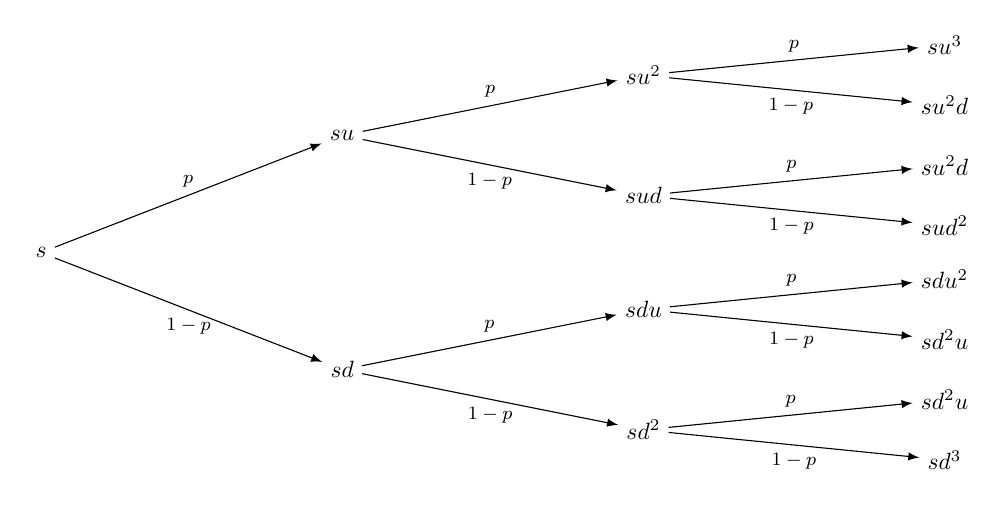
\begin{tikzpicture}[
    grow=right,
    scale=0.85, transform shape,
    level distance=45mm,
    level 1/.style={sibling distance=35mm},
    level 2/.style={sibling distance=18mm},
    level 3/.style={sibling distance=9mm},
    edge from parent/.style={draw, -latex},
    every node/.style={align=center}
]

  \node {$s$}
    child {
        node {$sd$}
        child {
            node {$sd^2$}
            child {
                node {$sd^3$}
                edge from parent node[below, font=\footnotesize] {$1-p$}
            }
            child {
                node {$sd^2u$}
                edge from parent node[above, font=\footnotesize] {$p$}
            }
            edge from parent node[below, font=\footnotesize] {$1-p$}
        }
        child {
            node {$sdu$}
            child {
                node {$sd^2u$}
                edge from parent node[below, font=\footnotesize] {$1-p$}
            }
            child {
                node {$sdu^2$}
                edge from parent node[above, font=\footnotesize] {$p$}
            }
            edge from parent node[above, font=\footnotesize] {$p$}
        }
        edge from parent node[below, font=\footnotesize] {$1-p$}
    }
    child {
        node {$su$}
        child {
            node {$sud$}
            child {
                node {$sud^2$}
                edge from parent node[below, font=\footnotesize] {$1-p$}
            }
            child {
                node {$su^2d$}
                edge from parent node[above, font=\footnotesize] {$p$}
            }
            edge from parent node[below, font=\footnotesize] {$1-p$}
        }
        child {
            node {$su^2$}
            child {
                node {$su^2d$}
                edge from parent node[below, font=\footnotesize] {$1-p$}
            }
            child {
                node {$su^3$}
                edge from parent node[above, font=\footnotesize] {$p$}
            }
            edge from parent node[above, font=\footnotesize] {$p$}
        }
        edge from parent node[above, font=\footnotesize] {$p$}
    };
\end{tikzpicture}
\end{center}



\vspace{1cm}

\noindent where

$A_1 = \{\omega \in \Omega \mid \omega_1 = w_u\}$

$A_2 = \{\omega \in \Omega \mid \omega_1 = w_d\}$

$B_1 = \{\omega \in \Omega \mid \omega_1 = w_u, \omega_2 = w_u\}$

$B_2 = \{\omega \in \Omega \mid \omega_1 = w_u, \omega_2 = w_d\}$

$B_3 = \{\omega \in \Omega \mid \omega_1 = w_d, \omega_2 = w_u\}$

$B_4 = \{\omega \in \Omega \mid \omega_1 = w_d, \omega_2 = w_d\}$

\vspace{0.5cm}

$\mathcal{J}_0 = \{\emptyset, \Omega\}, \quad \mathcal{J}_1 = \sigma(A_1, A_2), \quad \mathcal{J}_2 = \sigma(B_1, B_2, B_3, B_4)$

\vspace{1cm}

\noindent \textbf{T=3 Payoff}

\noindent Final Payoff

\section{Investment Strategies}

\begin{assumption}[Frictionless Market Assumption]
We assume the following idealized conditions:
\begin{enumerate}
\item No transaction costs,
\item Possibility of short selling,
\item Possibility of borrowing/lending at the same risk-free rate,
\item Perfect divisibility of assets,
\item No dividends (for simplicity).
\end{enumerate}
\end{assumption}




\begin{tcolorbox}[title=Reminder: Short Selling, colback=blue!5!white, colframe=blue!40!black]
A \textbf{short sale} consists of selling an asset that one does not own, hoping to buy it back later at a lower price.

\medskip
\textbf{Mechanism:}
\begin{enumerate}
    \item The investor ($C_1$) borrows the asset from a third party ($C_2$) through a broker.
    \item He immediately sells this asset on the market at the current price $S_t$.
    \item Later, he buys back the asset at price $S_{t+k}$ to return it (this is the unwinding).
\end{enumerate}

If $S_{t+k} < S_t$, he makes a profit. This is a bearish speculation strategy.

\begin{center}
\begin{tikzpicture}[
  >=Stealth, thick,
  scale=0.8, transform shape,
  circ/.style = {circle, draw, minimum size=14mm, align=center},
  elli/.style = {ellipse, draw, minimum width=30mm, minimum height=16mm, align=center}
]
% Nodes
\node[circ] (c1) {C$_1$};
\node[elli, right=2.8cm of c1] (brk) {Broker};
\node[circ, right=2.8cm of brk] (c2) {C$_2$};

% Arrows
\draw[->] (c1) to[bend left=20] node[midway, above=3pt, font=\small] {short sell} (brk);
\draw[->] (brk) to[bend left=20] node[midway, below=3pt, font=\small] {cash} (c1);

\draw[->] (brk) to[bend left=20] node[midway, above=3pt, font=\small] {borrow security} (c2);
\draw[->] (c2) to[bend left=20] node[midway, below=3pt, font=\small] {security} (brk);
\end{tikzpicture}
\end{center}
\end{tcolorbox}
Breakdown of the operation:
\begin{itemize}
  \item $C_1$ profits if the asset price decreases;
  \item $C_2$ and the broker receive fees;
  \item $C_2$ continues to receive dividends (if any) and can terminate the loan at any time.
\end{itemize}


\section{Financial Strategies and Self-Financing Portfolios}

\begin{definition}[Financial Strategy]
A \textbf{financial strategy} (or investment strategy) is a predictable stochastic process $(\hat H_t)_{t=1,\ldots,T}$ with values in $\RR^{d+1}$:
\begin{equation}
\hat H_t = (\hat H_t^0, \hat H_t^1, \ldots, \hat H_t^d),
\end{equation}
where $\hat H_t^j$ represents the quantity of asset $j$ held in the portfolio over the interval $]t-1, t]$.

The \textbf{portfolio value} (or wealth) at time $t$ is given by:
\begin{equation}
\hat V_t = \langle \hat H_t, \hat S_t \rangle = \sum_{k=0}^d \hat H_t^k \hat S_t^k.
\end{equation}
\end{definition}

\begin{remark}
The previous definition follows from the \emph{frictionless} assumption.
\end{remark}

\begin{definition}[Consumption Process]
Let $(\hat H_t)_{t\in\{0,\ldots,T\}}$ be a financial strategy.  
We define the \textbf{consumption process} $(\hat C_t)_{t\in\{1,\ldots,T\}}$ by:
\[
-\hat C_t = \hat V_t - \langle \hat H_{t-1}, \hat S_t \rangle,
\]
where $\langle \hat H_{t-1}, \hat S_t \rangle$ represents the value of the ``old'' portfolio at time $t$.

A financial strategy is said to be \textbf{self-financing} if, for all $t\in\{1,\ldots,T\}$,
\[
\hat C_t = 0.
\]
\end{definition}

\medskip

In this case, between $0$ and $T$, one does not have the right to consume or invest.  
One can only readjust the portfolio while respecting the budget constraint at each instant.

\begin{example}
If one invests at time $t=0$ and does nothing until maturity $T$, one implements a \emph{self-financing} strategy.
\end{example}

\begin{lemma}
A financial strategy can be characterized by $(\hat V_0, (\hat C_t)_{t\in\{1,\ldots,T\}}, (\hat H_t)_{t\in\{0,\ldots,T\}})$.
\end{lemma}

\begin{remark}
The lemma formalizes the link between financial flows (buying, selling, consumption) and portfolio composition.
The idea is that at each period $t$, we want to know:
\begin{itemize}
    \item how much of each asset we have (the vector $\hat H_t$);
    \item how much the portfolio is worth ($\hat V_t$);
    \item how much we withdraw or add (consumption $\hat C_t$ or capital injection).
\end{itemize}
The lemma states that the data of the initial value, the consumption process (how much is taken out of the portfolio at each date) and the risky strategy (how risk is allocated) is sufficient to completely reconstruct the strategy, including the portion invested in the risk-free asset (which serves as an adjustment or financing account).
\end{remark}


\begin{proof}
We denote $\hat S_t=(\hat S_t^0,\hat S_t^1,\ldots,\hat S_t^d)$ the price vector at time $t$ (non-discounted),
$\hat H_t=(\hat H_t^0,\ldots,\hat H_t^d)$ the strategy, and
\[
\hat V_t \;=\; \langle \hat H_t,\hat S_t\rangle \;=\; \sum_{k=0}^d \hat H_t^k\,\hat S_t^k
\]
the portfolio value at time $t$.
The \emph{consumption process} $(\hat C_t)_{t=1,\ldots,T}$ is defined by
\begin{equation}\label{eq:consumption-def}
-\hat C_t \;=\; \hat V_t - \langle \hat H_{t-1}, \hat S_t\rangle
\qquad (t=1,\ldots,T),
\end{equation}
that is: we start from the value of the old portfolio after the price movement,
we consume $\hat C_t$ (positive = withdrawal, negative = contribution), then we reallocate to obtain $\hat H_t$.

\smallskip
\noindent\textbf{Step 1 ($t=0$).}
By definition,
\[
\hat V_0 \;=\; \sum_{k=0}^d \hat H_0^k\,\hat S_0^k
\;=\; \hat H_0^0\,\hat S_0^0 \;+\; \sum_{k=1}^d \hat H_0^k\,\hat S_0^k.
\]
Isolating the risk-free component, we immediately obtain
\[
\hat H_0^0 \;=\; \frac{\hat V_0 - \sum_{k=1}^d \hat S_0^k\,\hat H_0^k}{\hat S_0^0}.
\]

\smallskip
\noindent\textbf{Step 2 ($t\ge 1$).}
The budget constraint at time $t$ is obtained by rewriting \eqref{eq:consumption-def}:
\[
\hat V_t \;=\; \langle \hat H_{t-1}, \hat S_t\rangle - \hat C_t.
\]
Now $\hat V_t=\langle \hat H_t,\hat S_t\rangle = \hat H_t^0\,\hat S_t^0 + \sum_{k=1}^d \hat H_t^k\,\hat S_t^k$,
so that
\[
\hat H_t^0\,\hat S_t^0 \;+\; \sum_{k=1}^d \hat H_t^k\,\hat S_t^k
\;=\; \langle \hat H_{t-1}, \hat S_t\rangle \;-\; \hat C_t.
\]
Isolating $\hat H_t^0$, we obtain the announced formula:
\[
\hat H_t^0 \;=\; \frac{-\hat C_t + \langle \hat H_{t-1}, \hat S_t\rangle - \sum_{k=1}^d \hat H_t^k\,\hat S_t^k}{\hat S_t^0},
\qquad t=1,\ldots,T.
\]

\smallskip
\noindent\textbf{Conclusion (characterization).}
The identities above show that, once we fix
$\hat V_0$, the consumption process $(\hat C_t)$ and the risky components
$(\hat H_t^1,\ldots,\hat H_t^d)$ for each $t$, the risk-free component $\hat H_t^0$
is entirely determined for $t=0$ and then recursively for $t\ge 1$.
Thus, the triplet $(\hat V_0,(\hat C_t),(\hat H_t))$ completely characterizes the financial strategy.
\end{proof}

\begin{corollary}
A self-financing financial strategy can be characterized by $(\hat V_0, (\hat H_t)_{t\in\{0,\ldots,T\}})$.
\end{corollary}

\begin{definition}[Discounted Values]
For all $k\in\{0,\ldots,d\}$, we define the \textbf{discounted values} by:
\[
S_t^k = \frac{\hat S_t^k}{\hat S_t^0}, \qquad V_t = \frac{\hat V_t}{\hat S_t^0}.
\]
Thus, $S_t^0 \equiv 1$ and $S_t = (S_t^1,\ldots,S_t^d)$ represents the vector of risky assets only.
\end{definition}

\begin{lemma}

\emph{A financial strategy is self-financing}
\[
\Longleftrightarrow\;
\forall\, t \in \{1,\ldots,T\},\quad
V_t = V_0 + \sum_{k=0}^{t-1} \langle H_k,\, S_{k+1} - S_k \rangle.
\]
\end{lemma}



\begin{proof}
By definition, for all $t\in\{0,\ldots,T\}$:
\[
\hat V_t = \hat H_t^0 \hat S_t^0 + \sum_{k=1}^d \hat H_t^k \hat S_t^k = \langle \hat H_t, \hat S_t \rangle.
\]

The self-financing condition gives:
\[
\hat V_t = \hat H_{t-1}^0 \hat S_t^0 + \sum_{k=1}^d \hat H_{t-1}^k \hat S_t^k = \hat H_{t-1}^0 \hat S_t^0 + \langle \hat H_{t-1}, \hat S_t \rangle.
\]
Thus,
\[
V_t = V_{t-1} + \langle H_{t-1}, S_t - S_{t-1} \rangle,
\]
and by induction:
\[
V_t = V_0 + \sum_{k=0}^{t-1} \langle H_k, S_{k+1} - S_k \rangle.
\]
\end{proof}

\begin{remark}
The variation in portfolio value is entirely attributable to the variation in asset prices when the strategy is self-financing (i.e., without consumption).
\end{remark}

\begin{remark}
We denote:
\[
(H \cdot S)_t = \sum_{k=0}^{t-1} \langle H_k, S_{k+1} - S_k \rangle,
\]
which corresponds to the discrete stochastic integral of process $H$ with respect to $S$.
\end{remark}


\section{Contingent Claims and Attainability Sets}

A contingent claim (or derivative asset) is a financial contract whose value at a future date $T$ depends on the future state of the world. Mathematically, it is a random variable $\hat{U}$ that is $\mathcal{F}_T$-measurable. Its discounted value is denoted $U = \hat{U} / S^0_T$. The central question of the theory is whether one can "attain" this claim with a given initial cost.

\begin{itemize}
    \item \textbf{Replicable claim:} A claim $\hat{U}$ is said to be replicable at price $a$ if there exists a self-financing financial strategy $(H_t)$ such that the initial investment is $\hat{V}_0 = a$ and the final portfolio value exactly matches the claim's payoff, $\hat{V}_T = \hat{U}$.
    \item \textbf{Set $K_a$:} This set represents all final payoffs (discounted) that can be attained with an initial cost $a$. Formally:
    \[
    K_a = \{ a + (H \cdot S)_T \mid H \in \mathcal{H}^d \}
    \]
    where $\mathcal{H}^d$ is the set of predictable strategies on the risky assets. The set $K = K_0$ is particularly important: it represents the set of net gains attainable at zero initial cost.
    \item \textbf{Set $\mathcal{C}_a$:} This set represents all claims (discounted) that can be super-replicated with an initial cost $a$, meaning their payoff is dominated by an attainable payoff:
    \[
    \mathcal{C}_a = \{ U \in L^\infty(\mathcal{F}_T) \mid \exists g \in K_a, g \ge U \}
    \]
    The set $\mathcal{C} = \mathcal{C}_0$ corresponds to claims super-replicable at zero cost.
    \item \textbf{Properties of $K$ and $\mathcal{C}$:} These sets have fundamental geometric structures for what follows.
    \begin{itemize}
        \item $K$ is a vector space (closed in finite dimension).
        \item $\mathcal{C}$ is a convex cone (closed in finite dimension).
    \end{itemize}
    These geometric properties are fundamental because they validate the application of Hahn-Banach separation theorems, which constitute the cornerstone of the proof of the Fundamental Theorem of Arbitrage.
\end{itemize}

\section{Arbitrage Opportunities}

\begin{definition}[Arbitrage Opportunity]
A self-financing strategy $(\hat H_t)_{t\in[0,T]}$ is an \emph{arbitrage opportunity} (A.O. hereafter) if
\begin{equation}
\hat V_0 = 0, \quad \hat V_T \ge 0 \ \text{P-a.s.}, \quad \text{and} \quad P(\hat V_T > 0) > 0.
\end{equation}
\end{definition}

\begin{remarks}
\item[(a)] In the previous definition, the condition above remains unchanged if the probability $P$ is replaced by a probability $Q$ such that $Q \sim P$.
\item[(b)] The following conditions are equivalent:
\begin{align}
& V_0 = 0, \; V_T \ge 0 \text{ P-a.s. and } P(V_T > 0) > 0 \\
\Longleftrightarrow \quad & V_0 = 0, \; (H \cdot S)_T \ge 0 \text{ P-a.s. and } P((H \cdot S)_T > 0) > 0 \\
\Longleftrightarrow \quad & V_0 = 0, \; V_T \ge 0 \text{ P-a.s. and } \E_P[V_T] > 0.
\end{align}
\end{remarks}

\paragraph*{Context of Attainability Sets}
The central objective of arbitrage theory is to determine whether a future "payoff", that is, a contingent claim such as an option, can be perfectly generated by a dynamic investment strategy. To formalize this idea, we introduce two fundamental sets. The set $K_a$ represents the universe of all possible financial outcomes (expressed in discounted value at the final date $T$) that can be attained starting from an initial capital $a$ and applying a self-financing strategy. The set $\mathcal{C}_a$, on the other hand, is broader: it groups all contingent claims that can at least be matched, that is, "super-replicated", with this same initial capital $a$. These geometric structures are the key to linking the absence of risk-free profit opportunities to the valuation of financial assets.

\begin{definition}[Contingent Claim]
\begin{enumerate}[label=(\alph*)]
\item A contingent claim $\hat U$ is a random variable measurable with respect to $\mathcal{F}_T$.  
In this case, we define its discounted value by
\begin{equation}
U = \frac{\hat U}{\hat S_T^0}.
\end{equation}

\item A contingent claim $\hat U$ is said to be \emph{replicable} (resp. \emph{super-replicable}) at price $a$ if there exists a self-financing portfolio $(\hat H_t)_{t\in[0,T]}$ such that
\begin{equation}
\hat V_0 = a \quad \text{and} \quad \hat V_T = \hat U \; (\text{resp. } \hat V_T \ge \hat U).
\end{equation}
We then denote
\begin{equation}
K_a = \bigl\{\, a + (H \cdot S)_T \;|\; H \in \mathcal{H}^d \,\bigr\},
\end{equation}
where $\mathcal{H}^d$ is the set of adapted stochastic processes with values in $\mathbb{R}^d$, and
\begin{equation}
\mathcal{C}_a = \bigl\{\, U \in L^\infty(\mathcal{F}_T) \;|\; \exists g \in K_a,\, g \ge U \,\bigr\}.
\end{equation}
\end{enumerate}
We always have $K_a \subset \mathcal{C}_a$.
\end{definition}

\begin{remarks}
\item[(a)] We denote $\mathcal{C} = \mathcal{C}_0$ and $K = K_0$. Thus, $\mathcal{C}_a = a + \mathcal{C}$ and $K_a = a + K$.

\item[(b)] $K$ is a vector space (hence convex and closed in finite dimension).

\item[(c)] $\mathcal{C}$ is a convex cone containing
\[
L_-^\infty(\Omega, \mathcal{F}_T, P) = \{\, X \in L^\infty \mid X \le 0 \text{ P-a.s.} \}.
\]
\end{remarks}

\begin{definition}[No-Arbitrage Assumption (NA)]
We say that the \emph{no-arbitrage} assumption (NA hereafter) is satisfied if there exists no arbitrage opportunity, that is:
\begin{equation}
\text{if } V_0 = 0, \; V_T \ge 0 \text{ P-a.s. } \Rightarrow P(V_T = 0) = 1.
\end{equation}
\end{definition}

\begin{tcolorbox}[title=Intuition: No Free Lunch, colback=red!5!white, colframe=red!50!black]
The NA assumption means that it is impossible to make money for sure without initial investment and without taking any risk of loss.
\begin{itemize}
    \item If I start from nothing ($V_0=0$) and can never lose ($V_T \ge 0$), then I cannot gain anything ($V_T=0$).
    \item This is the minimal condition for a financial model to be viable. Without it, prices would have no meaning (infinite supply/demand).
\end{itemize}
\end{tcolorbox}

\begin{lemma}
We have the following equivalences:
\begin{equation}
NA \;\Longleftrightarrow\; K \cap L_+^0(\Omega, \mathcal{F}_T, P) = \{0\}
\;\Longleftrightarrow\;
\mathcal{C} \cap L_+^0(\Omega, \mathcal{F}_T, P) = \{0\}.
\end{equation}
\end{lemma}

\begin{proof}
Direction ($NA \Rightarrow K \cap L^0_+ = \{0\}$): We reason by contradiction. Suppose that the no-arbitrage assumption (NA) is satisfied, but that there exists a non-zero element $g$ in the intersection $K \cap L^0_+$.
\begin{enumerate}
    \item Since $g \in K$, by definition, $g$ is the discounted final value $V_T$ of a self-financing strategy $H$ with initial cost $V_0 = 0$. So $g = (H \cdot S)_T$.
    \item Since $g \in L^0_+$, we have $g \ge 0$ P-a.s. (almost surely).
    \item Since $g$ is non-zero, $P(g > 0) > 0$.
    \item In summary, we have found a self-financing strategy with $V_0 = 0$, $V_T \ge 0$ P-a.s., and $P(V_T > 0) > 0$. This is precisely the definition of an arbitrage opportunity. However, we assumed NA. There is therefore a contradiction. The initial hypothesis is false, and therefore $K \cap L^0_+$ must be reduced to $\{0\}$.
\end{enumerate}

Direction ($K \cap L^0_+ = \{0\} \Rightarrow NA$): Suppose that $K \cap L^0_+ = \{0\}$. We must show that the NA assumption is satisfied.
\begin{enumerate}
    \item Consider any self-financing strategy $H$ such that $V_0 = 0$ and $V_T \ge 0$ P-a.s.
    \item By definition, the final value $V_T$ of such a strategy belongs to $K$.
    \item Since $V_T \ge 0$, $V_T$ also belongs to $L^0_+$.
    \item Therefore, $V_T$ belongs to the intersection $K \cap L^0_+$.
    \item By our hypothesis, this intersection is reduced to $\{0\}$. This implies that $V_T = 0$ P-a.s. This corresponds exactly to the definition of the no-arbitrage assumption (NA): any strategy starting from zero and that can only generate gains cannot actually generate any gain.
\end{enumerate}

This mathematical reformulation of the no-arbitrage condition is the key that will allow us to mobilize the tools of functional analysis to prove the Fundamental Theorem of asset pricing.
\end{proof}

\begin{definition}[Local Arbitrage]
Let $t \in \{1, \dots, T\}$.  
A \emph{local arbitrage at $t$} is a random variable $\xi$ measurable with respect to $\mathcal{F}_{t-1}$, with values in $\mathbb{R}^d$, such that:
\[
\langle \xi, S_t - S_{t-1} \rangle \ge 0 \text{ P-a.s.}, 
\quad \text{and} \quad P\bigl( \langle \xi, S_t - S_{t-1} \rangle > 0 \bigr) > 0.
\]
The market satisfies condition $NA(t)$ if there exists no local arbitrage at $t$.
\end{definition}

\begin{lemma}
\[
NA \;\Longleftrightarrow\; NA(t) \quad \forall t \in \{1, \dots, T\}.
\]
\end{lemma}

\begin{proof}[Proof of the lemma: $NA \Longleftrightarrow NA(t)\ \forall t$]
\subsection*{Direction $\Rightarrow$:}
Suppose that the global no-arbitrage assumption (NA) is satisfied.  
If there existed a local arbitrage at some $t \in \{1,\ldots,T\}$, then one could construct a self-financing strategy $(H_s)_{s\in[0,T]}$ such that
\[
V_0 = 0, \qquad 
V_T = \langle \xi, S_t - S_{t-1} \rangle \ge 0 \text{ a.s.}, \qquad 
\mathbb{P}(V_T > 0) > 0.
\]
This strategy would constitute a global arbitrage opportunity, which would contradict (NA).  
Thus, if (NA) is true, no local arbitrage can exist:
\[
NA \;\Rightarrow\; NA(t), \quad \forall t\in\{1,\ldots,T\}.
\]

\subsection*{Direction $\Leftarrow$:}
We show the converse by induction on the number of periods $T$ of the market.

\subsubsection*{Base Case}
For $T=1$, the result is obvious: a global arbitrage over a single period is exactly a local arbitrage.

\subsubsection*{Induction Hypothesis}
Suppose the result is true for a market of maturity $T-1$, that is:
\[
\text{in a market with $T-1$ periods,} \qquad
NA \;\Leftarrow\; NA(t), \quad \forall t \in \{1,\ldots,T-1\}.
\]

\subsubsection*{Induction Step}
Consider a market with $T$ periods and reason by contraposition.  
Let $(\hat H_t)_{t=0}^T$ be an arbitrage opportunity (A.O.) on $[0,T]$.  
We then have:
\[
V_T = V_{T-1} + \langle H_{T-1}, S_T - S_{T-1} \rangle, 
\qquad V_T \ge 0,\quad \mathbb{P}(V_T > 0) > 0.
\]
Let us introduce the set and the random variable:
\[
A = \{ V_{T-1} < 0 \} \in \mathcal{F}_{T-1},
\qquad
\xi = H_{T-1}\mathbf{1}_A \quad (\mathcal{F}_{T-1}\text{-measurable}).
\]
Then:
\[
\mathbf{1}_A V_T
= \mathbf{1}_A V_{T-1}
+ \big\langle \mathbf{1}_A H_{T-1},\, S_T - S_{T-1} \big\rangle
\ge 0.
\]

\textbf{Case 1:} If $\mathbb{P}(A) > 0$, then $\xi$ defines a local arbitrage because
\[
\langle \xi, S_T - S_{T-1} \rangle \ge 0 \text{ a.s.}, 
\qquad 
\mathbb{P}(\langle \xi, S_T - S_{T-1} \rangle > 0) \ge \mathbb{P}(A) > 0.
\]

\textbf{Case 2:} If $\mathbb{P}(A) = 0$, then $V_{T-1} \ge 0$ a.s.  
Two sub-cases arise:
\[
\begin{cases}
(1) & V_{T-1} = 0\ \text{a.s.} 
\quad \Rightarrow\ H_{T-1}\ \text{is a local arbitrage at } T, \\[0.5em]
(2) & \mathbb{P}(V_{T-1}>0) > 0 
\quad \Rightarrow\ (H_t)_{t\le T-1}\ \text{is an A.O. on } [0,T-1].
\end{cases}
\]
In the second sub-case, the induction hypothesis applies: there exists a local arbitrage 
at some $t \in \{1,\ldots,T-1\}$.

Thus, in all cases, a global A.O. on $[0,T]$ implies the existence of a local arbitrage.  
We deduce:
\[
NA(t)\ \forall t \;\Rightarrow\; NA.
\]

\textbf{Conclusion:} both directions are thus established, and we indeed have
\[
NA \;\Longleftrightarrow\; NA(t), \quad \forall t\in\{1,\ldots,T\}.
\]
\end{proof}
